%% Sample chapter 1
%%=========================================

\chapter{Introduction}
The Oxford English Dictionary defines ``digitization" as the action or process of digitizing. Digitizing means the conversation of analogue data into digital form\cite{oed-digitization}. As the world grows more and more digital, the need to digitize increases proportioned. Countless research documents and theses are written in the field of optical character recognition. OCR is the task of identifying printed characters and symbols using computer software. This task is critical in the digitization process.

\section{Context}
TODO

\section{Personal motivation}
TODO

\section{Goals}
The goal is to make OCR possible in a very limited search space. Several papers are already written on this field and mostly deals with symbols that are ``damaged" or are missing some part of the...

\subsection{Example of use}
Markus ``Notch" Persson is a Swedish video game programmer and designer. He is most famous for crating the highly praised game Minecraft. During development of the game, Persson was a inveterate user of Twitter, and used to hint or tease upcoming features of the game. On June 12th 2011, Persson Tweeted the following Tweet:

\begin{figure}[h]
    \centering
    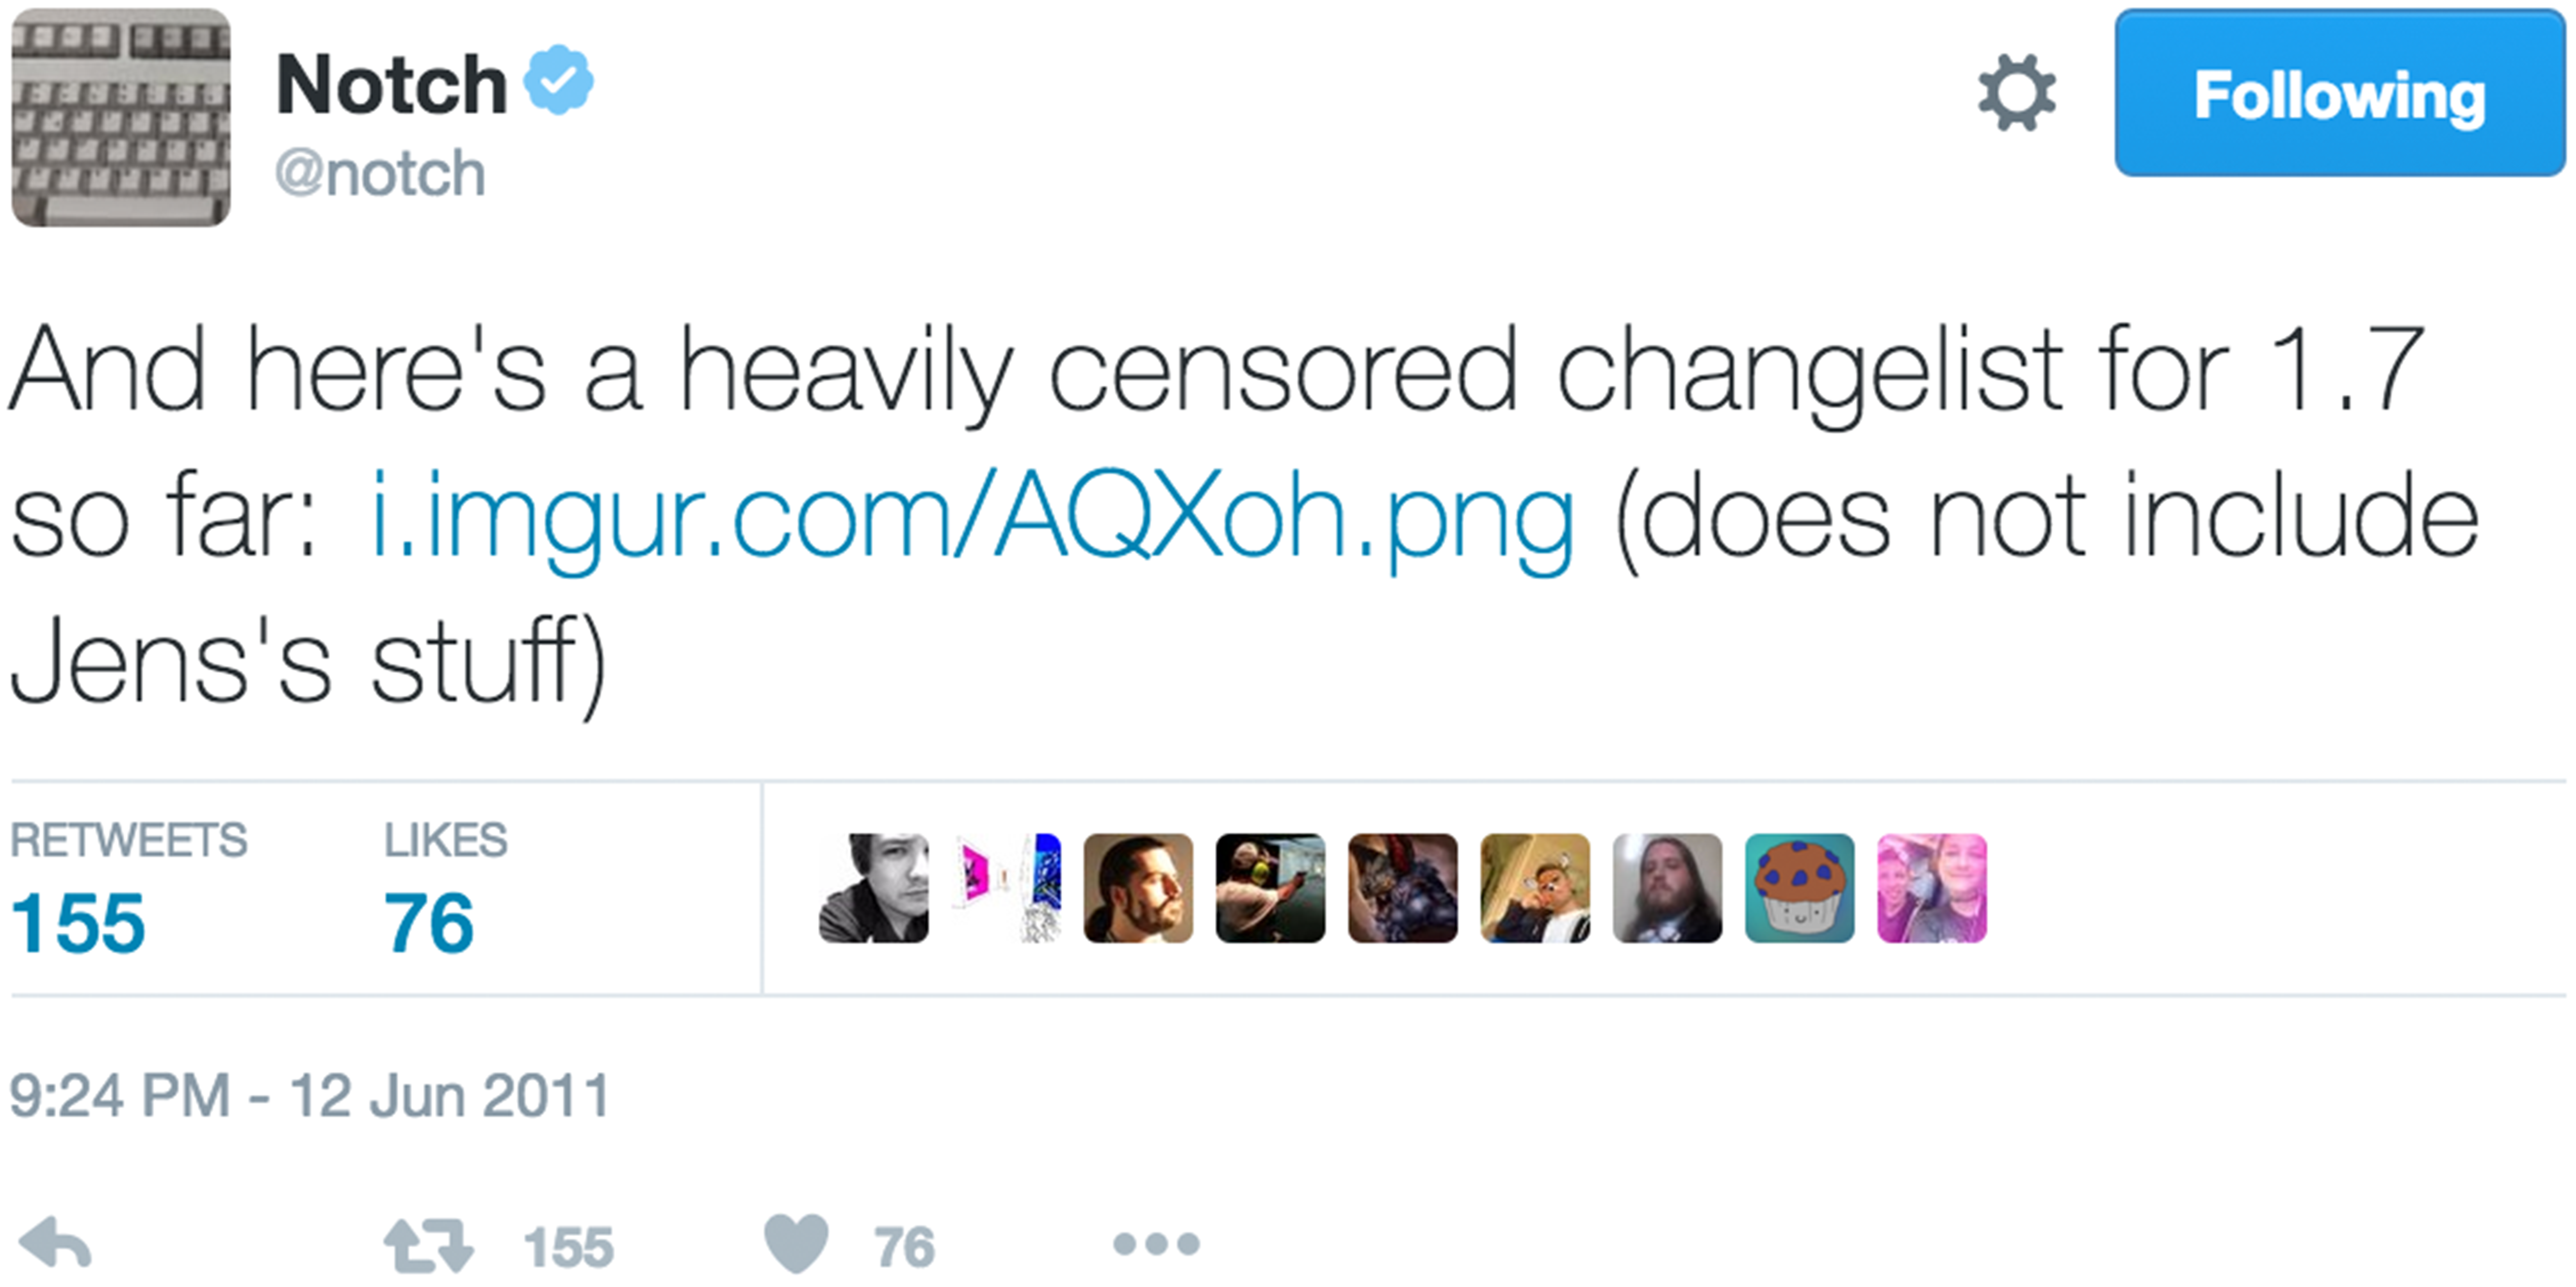
\includegraphics[width=0.7\textwidth]{fig/chapter1/notch_tweet.png}
    \caption{Print screen of Tweet from notch\footnotemark}
\end{figure}
\footnotetext{Tweet and image used with the consent of Markus Persson. \url{https://twitter.com/notch/status/790531003169341440}}

The image he is referring to looks like this:

\begin{figure}[h]
    \centering
    \includegraphics[width=0.7\textwidth]{fig/chapter1/notch_eclipse.png}
    \caption{Blurred image of Minecraft 1.7 changelog from @notch's Tweet}
\end{figure}

The image looks like it is taken inside a text editor or \gls{IDE}. There is a file currently opened, with several other files, or tabs, partially visible at the top of the image. The file that is corrently opened seems to be a changelog for the upcoming 1.7 version of Minecraft, with the new major version written on the first line, followed by a list of changed. The content is mostly burred out, showing only parts of the first letter on each line and the content of some longer lines. The image is also cropped so that the file names for the files that are currently opened in the project is not displayed.

\section{Structure and approach}
TODO